\documentclass[a4paper,12pt]{article} % тип документа

%  Русский язык
\usepackage[T2A]{fontenc}			% кодировка
\usepackage[utf8]{inputenc}			% кодировка исходного текста
\usepackage[english,russian]{babel}	% локализация и переносы

\usepackage{graphicx}               % импорт изображений
\usepackage{wrapfig}                % обтекаемые изображения
\graphicspath{{pictures/}}          % обращение к подкаталогу с изображениями
\usepackage[14pt]{extsizes}         % для того чтобы задать нестандартный 14-ый размер шрифта
\usepackage{amsfonts}               % буквы с двойными штрихами
\usepackage[warn]{mathtext}         % русский язык в формулах
\usepackage{indentfirst}            % indent first
\usepackage[margin = 25mm]{geometry}% отступы полей
\usepackage{amsmath}                % можно выводить фигурные скобочки -- делать системы уравнений
\usepackage[table,xcdraw]{xcolor}   % таблицы
\usepackage{amsmath,amsfonts,amssymb,amsthm,mathtools} % Математика
\usepackage{wasysym}                % ???
\usepackage{upgreek}                % ???  
\usepackage{caption}
\captionsetup{labelsep=period}
\usepackage{gensymb} % degree symbol

\begin{document}
	\begin{center}
		
		\normalsize{Федеральное государственное автономное образовательное учреждение высшего образования}
		
		\textbf{НАЦИОНАЛЬНЫЙ ИССЛЕДОВАТЕЛЬСКИЙ УНИВЕРСИТЕТ \\ <<МОСКОВСКИЙ ФИЗИКО-ТЕХНИЧЕСКИЙ ИНСТИТУТ>>}
		\vspace{13ex}
		
		\textbf{Лабораторная работа 2.1.1 \\ <<Измерение удельной теплоемкости воздуха при постоянном давлении>> }
		\vspace{40ex}
		
		\normalsize{Овсянников Михаил Александрович \\ студент группы Б01-001\\ 1 курс ФРКТ\\}
	\end{center}
	
	\vfill 
	
	\begin{center}
		г. Долгопрудный\\ 
		2021 г.
	\end{center}
	
	\thispagestyle{empty} % выключаем отображение номера для этой страницы
	
	\newpage
	
	\textbf{Цель работы:} 1) измерение повышения температуры воздуха в результате подвода тепла при стационарном течении через стеклянную трубу; 2) вычисление по результатам измерений теплоемкости воздуха при постоянном давлении.
	\\
	\\
	\indent	\textbf{В работе используются:} теплоизолированная трубка; электронагреватель; источник питания постоянного тока Б5-47; термопара; амперметр; вольтметр; универсальный цифровой вольтметр В7-23; газовый счетчик; секундомер.
	
	\section*{Теоретические сведения}
Определение теплоемкости тел обычно производится в калориметрах, т. е. в сосудах, обеспечивающих теплоизоляцию исследуемого тела от внешней среды. При этом регистрируется количество тепла $\delta Q$, полученное телом, и изменение температуры этого тела $dT$. Теплоемкость определяется как частное от деления $\delta Q$ на $dT$:

\begin{equation*}
	C = \frac{\delta Q}{dT}.
\end{equation*}


Надежность измерения определяется в основном качеством калориметра. Необходимо, чтобы количество тепла, затрачиваемое на нагревание исследуемого тела, было существенно больше тепла, расходуемого на нагревание калориметра, и на потери, связанные с утечкой тепла из установки. При измерении теплоемкости воздуха эти требования выполнить очень трудно, так как масса воздуха, заключенного в калориметре, и, следовательно, количество тепла, идущее на его нагревание, очень малы. Чтобы увеличить количество воздуха при неизменных размерах установки, в нашей работе воздух продувается сквозь калориметр, внутри которого установлен нагреватель. Измеряется количество тепла, отдаваемое нагревателем, масса протекающего воздуха и изменение его температуры.

\section*{Экспериментальная установка.}
Схема установки изображена на рисунке 1. Кран К служит для регулировки количества воздуха, поступающего в установку. Объем воздуха, прошедшего через калориметр, измеряется газовым счетчиком ГС.

\begin{figure}
	\centering
	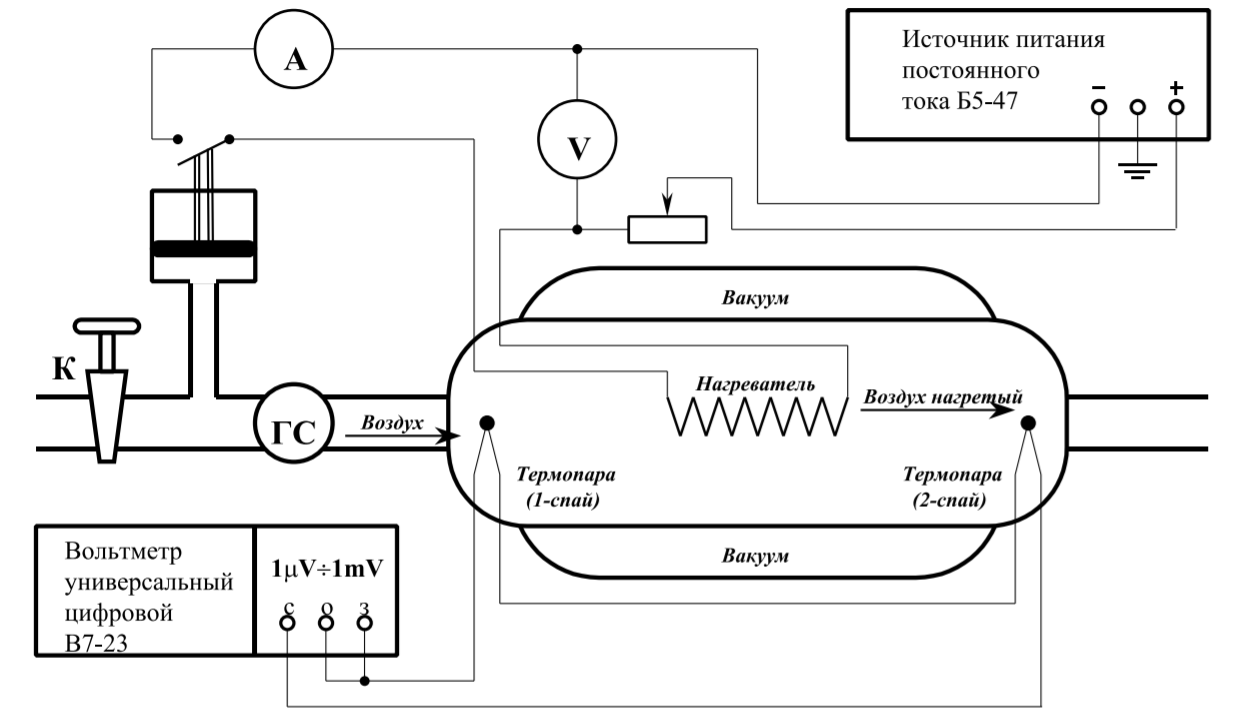
\includegraphics[scale=0.5]{Рис1.png}
	\caption{Схема экспериментальной установки}
\end{figure}


Калориметр представляет собой стеклянную трубку с вакуумной термоизолирующей оболочкой. Давление воздуха в вакуумной оболочке калориметра не превышает $10^{-5}$ торр. Теплопроводность воздуха при таком давлении ничтожно мала. Обращенные в сторону вакуума стенки калориметра посеребрены, что уменьшает потери тепла из-за излучения.


Электронагреватель, укрепленный в калориметре, сделан в виде сетки и подключен к источнику питания постоянного тока Б5-47. В процессе измерений нагреватель обдувается проходящим через калориметр воздухом и равномерно нагревает его. Для предохранения электропечи от перегорания предусмотрена блокировка, размыкающая цепь нагревателя при отключении воздушного потока или при недостаточной его скорости. В цепь нагревателя включены амперметр и вольтметр, служащие для измерения мощности протекающего через нагреватель тока. Для измерения температуры воздуха служит термопара. Один спай термопары расположен в струе воздуха, входящего в калориметр, второй спай — в струе выходящего нагретого воздуха. Возникающая в термопаре ЭДС пропорциональна изменению температуры воздуха и измеряется универсальным цифровым вольтметром В7-23. В работе применяется медно-константановая термопара. При разности температур спаев 100 $\degree$C ЭДС термопары равна 4,23 мВ (холодный спай находится при комнатной температуре).


В начале опыта, непосредственно после включения установки, значительная часть мощности нагревателя расходуется на нагревание калориметра. Через некоторое время распределение температур устанавливается, и мощность затрачивается на нагревание воздуха и на потери, связанные главным образом с теплопроводностью стенок.


Отметим, что потери тепла зависят только от распределения температур вдоль стенок, а значит, от перепада температур на спаях термопары, и не зависят непосредственным образом от мощности нагревателя и потока воздуха. Это обстоятельство позволяет экспериментальным путем найти и исключить потери тепла в калориметре.


Вычислим работу, совершаемую при протекании газа через калориметр. Внешняя работа по перемещению моля газа в направлении течения в начале трубки равна $A_{1} = P_{1}V_{1}$, а в конце трубки давление препятствует движению и внешняя работа над газом отрицательна: $A_{2} = -P_{2}V_{2}$. Полная работа над газом равна $A_{1} + A_{2} = P_{1}V_{1} - P_{2}V_{2}$, а работа самого газа равна этой же величине, но с обратным знаком:


\begin{equation*}
	A = P_{2}V_{2} - P_{1}V_{1}.
\end{equation*}


\noindent Здесь $P_{1}, V_{1}$ — давление и объем моля газа на входе, а $P_{2}, V_{2}$, — соответственно на выходе трубки. 


Внутренняя энергия газа изменяется на величину $\Delta U = U_{2} - U_{1}$.


Для определения количества тепла $Q$ , полученного газом, воспользуемся первым началом термодинамики, то есть уравнением:

\begin{equation*}
	Q = U_{2} - U_{1} + P_{2}V_{2} - P_{1}V_{1} = H_{2} - H_{1},
\end{equation*}


\noindent где $H = U + PV$ — энтальпия. Подведенное тепло идет на увеличение энтальпии (необходимо отметить, что в данном эксперименте можно пренебречь изменением кинетической энергии газа из-за малости скорости движения газа по сравнению со скоростью звука).


Для идеального газа $H = C_{p}T$, поэтому


\begin{equation*}
	Q = C_{p}(T_{2} - T_{1}).
\end{equation*}


\noindent Следовательно, в данном эксперименте измеряется теплоемкость при постоянном давлении — это результат стационарности процесса.


Расчет удельной теплоемкости воздуха производится по очевидной формуле:


\begin{equation}
	c_{p} = \frac{Q}{m\Delta T} = \frac{IV - N}{m\Delta T},
\end{equation}


\noindent где $IV$ — мощность, выделяемая нагревателем, $N$ — мощность тепловых потерь, $m$ — масса воздуха, проходящего через калориметр за единицу времени, $\Delta T$ — разность температур, измеренная термопарой.

\end{document}